% Clase
\documentclass[11pt,a4paper,spanish,twoside]{book}

% Órdenes auxiliares
% Español
\usepackage[spanish]{babel}
\usepackage[utf8]{inputenc}

\usepackage{lmodern}
\usepackage[T1]{fontenc}
%\usepackage{textcomp}
%\usepackage{times}

% Símbolo del euro
\usepackage{textcomp}

%Profundidad de numeración
\setcounter{secnumdepth}{3}

% Imágenes
\usepackage[pdftex]{graphicx}
\usepackage{latexsym}
\usepackage{fancybox}

% Tablas
\usepackage{array}

% Enumeraciones
\usepackage{enumerate}

% Ruta para las imágenes
\graphicspath{{img/}}

% Rotaciones
\usepackage[twoside]{rotating}

% Multirow
\usepackage{multirow}

% Referencias
\usepackage[spanish]{varioref}
\usepackage[pdftex,colorlinks=true,linkcolor=black]{hyperref}

% Colores
\usepackage{color}
\usepackage{colortbl}

% Párrafos
\setlength{\parskip}{6pt}

% Code for creating empty pages
% No headers on empty pages before new chapter
\makeatletter
\def\cleardoublepage{\clearpage\if@twoside \ifodd\c@page\else
    \hbox{}
    \thispagestyle{empty}
    \newpage
    \if@twocolumn\hbox{}\newpage\fi\fi\fi}
\makeatother \clearpage{\pagestyle{empty}\cleardoublepage}

%Para las secciones y las subseciones de las actas
\makeatletter
\renewcommand{\section}{%
  \@startsection{section}{1}{0mm}{\baselineskip}%
  {0.1mm}{\large\bf}%
}%
\renewcommand{\subsection}{%
  \@startsection{subsection}{2}{0mm}{2mm}%
  {0.1mm}{\normalsize\bf}%
}%
\renewcommand{\subsubsection}{%
  \@startsection{subsubsection}{3}{0mm}{2mm}%
  {0.1mm}{\normalsize\bf\emph}%
}%
\makeatother
\usepackage{titlesec}

\titleformat{\chapter}[display]
  {\bfseries\Large}
  {\filleft\MakeUppercase{\chaptertitlename} \Huge\thechapter}
  {4ex}
  {\titlerule
   \vspace{2ex}%
   \filright}
  [\vspace{2ex}%
   \titlerule]

% Fancyhdr - Encabezados y pies de página
\usepackage{fancyhdr}
% Márgenes
\headsep=8mm
\footskip=14mm

% Fancy Header Style Options
\pagestyle{fancy}               % Sets fancy header and footer
\fancyfoot{}                    % Delete current footer settings

% Sin mayúsculas en la cabecera
\lhead{\nouppercase{\rightmark}}
\rhead{\nouppercase{\leftmark}}

% Capítulo
\renewcommand{\chaptermark}[1]{ % Lower Case Chapter marker style
  \markboth{\chaptername\ \thechapter.\ #1}{}} 

% Sección
\renewcommand{\sectionmark}[1]{ % Lower case Section marker style
  \markright{\thesection.\ #1}} 

% Página
\fancyhead[LE,RO]{\bfseries\thepage} % Page number (boldface) in left on even
                                     % pages and right on odd pages

% ------------------ Macro para encabezados y pies de página-------------------
%    Uso: \encabezado{pares(pag izquierda)}
% -----------------------------------------------------------------------------
\def\encabezado{
  \fancyhead[RE]{\bfseries\leftmark}     % In the right on even pages
  \fancyhead[LO]{\bfseries\rightmark}  % In the left on odd pages
  \renewcommand{\headrulewidth}{0.5pt} % Width of head rule
}
% -----------------------------------------------------------------------------

% ------------------ Macro para insertar una imagen ---------------------------
%    Uso: \imagen{nombreFichero}{Ancho(cm))}{Etiqueta}{Identificador}
% -----------------------------------------------------------------------------
\usepackage{float}
\usepackage{ifthen}
\def\imagen#1#2#3#4{
  \begin{figure}[H]
    \begin{center}
      \ifthenelse{\equal{#2}{}}
      {\includegraphics{#1}}{\resizebox{#2cm}{!}{\includegraphics{#1}}}
      \ifthenelse{\equal{#3}{}}{}{\caption{#3}}
      \label{#4}
    \end{center}
  \end{figure}
}
% -----------------------------------------------------------------------------


% ------------------ Macro para la portada ------------------------------------
%    Uso: \portada{asignatura}{titulo}{subtítulo}{autor}{fecha}
% -----------------------------------------------------------------------------
\def\portada#1#2#3#4#5{
  \thispagestyle{empty}
  \vspace*{-3.3cm}

  \begin{minipage}[t]{14cm}
    \begin{center}
      
\includegraphics[scale=0.25]{logo}
  
      \vspace*{1.5cm}
      {\Large \textbf{Universidad de Castilla-La Mancha\\ 
          Escuela Superior de Informática}\\}
    
      \vspace*{1.2cm}
      {\huge \textbf{#1}\\}
    
      \vspace*{1.5cm}
      {\huge #2\\}{\Large #3\\}
    
      \vspace*{1.5cm}
      {\large #4\\}
      \vspace*{1.4cm}
      \large{#5}
    \end{center}
  \end{minipage}

  \newpage
%   \vspace*{1cm}
%   \thispagestyle{empty} 
%   \newpage
}
% -----------------------------------------------------------------------------


% ------------------ Macro para la licencia -----------------------------------
%    Uso: \portada{asignatura}{titulo}{subtítulo}{autor}{fecha}
% -----------------------------------------------------------------------------
\def\licencia#1{
  \thispagestyle{empty}  % Suprime la numeración de esta página
  \vspace*{16.5cm}
  \begin{small}
    \copyright~ #1. Se permite la copia, distribución y/o 
    modificación de este documento bajo los términos de la licencia de
    documentación libre GNU, versión 1.1 o cualquier versión posterior publicada
    por la {\em Free Software Foundation}, sin secciones invariantes. Puede
    consultar esta licencia en http://www.gnu.org. \\[0.2cm]
    Este documento fue compuesto con \LaTeX{}. 
  \end{small}
  \newpage
%   \thispagestyle{empty}
%   \vspace*{0cm}
%   \newpage
}
% -----------------------------------------------------------------------------




\usepackage{amsthm}
\usepackage{verbatim}
\usepackage{multirow}

%Para las secciones y las subseciones
\makeatletter
\renewcommand{\section}{
  \@startsection{section}{1}{0mm}{\baselineskip}
  {2.5mm}{\Large\bf}
}
\renewcommand{\subsection}{
  \@startsection{subsection}{2}{0mm}{2mm}
  {4.0mm}{\bf}
}
\renewcommand{\subsubsection}{
  \@startsection{subsubsection}{3}{0mm}{2mm}
  {0.1mm}{\normalsize\bf\emph}
}
\makeatother

\theoremstyle{plain} \newtheorem{nota}{Nota}

% Encabezado y pie de página
\encabezado

\begin{document}

% Portada
\portada{Procesadores de Lenguaje}
{$1^{er}$ Trabajo en grupo}{Analizador sintáctico descendente LL1\\Resolución}
{Alicia Martín-Benito Escalona\\Juan Miguel Torres Triviño}{25 de Noviembre de 
2011}  

% Licencia
\licencia{Alicia Martín-Benito Escalona, Juan Miguel Torres Triviño} 

% Índices
\tableofcontents
\listoftables
\listoffigures

\chapter{Resolución de conflictos}

\section{Resolución de recursividad a la izquierda}

Como se puede ver en el cuadro \ref{rec} se produce recursividad a la izquierda
en la producción del no terminal \emph{W}.
\begin{table}[!ht]
  \centering
  \begin{tabular}{lll}
    \hline
    W   & $\to$ & W , ACC | ACC\\
    \hline
  \end{tabular}
  \caption{Recursividad a la izquierda}\label{rec}
\end{table}

Este conflicto es el más simple de los que nos podemos encontrar en la gramática
y se resuelve haciendo uso de una producción auxiliar, por tanto la producción 
del no terminal \emph{W} se transforma en las producciones del cuadro 
\ref{rec1}.

\begin{table}[!ht]
  \centering
  \begin{tabular}{lll}
    \hline
    W   & $\to$ & ACC W'\\
    W'  & $\to$ & , W | $\varepsilon$\\
    \hline
  \end{tabular}
  \caption{Resolución de la recursividad a la izquierda}\label{rec1}
\end{table}

\section{Resolución del conflicto de iniciales}

Como se puede ver en el cuadro \ref{ini} se produce un conflicto entre iniciales
en la producción del no terminal \emph{ACC}.
\begin{table}[!ht]
  \centering
  \begin{tabular}{lll}
    \hline
    ACC & $\to$ & AC ( PE ) | AC ( POS , POS ) |\\
        &       & AC ( OBS , POS ) | AC ( OBS , POS , POS ) |\\
        &       & AC ( OBS , POS , U )\\
    \hline
  \end{tabular}
  \caption{Conflicto entre iniciales}\label{ini}
\end{table}

Para resolver este conflicto se utiliza la factorización, es decir, realizar un
patrón común de las producciones donde se produce el conflicto y generar una 
producción auxiliar con la opcionalidad de las partes que no son comunes. En 
nuestro caso al realizar una primera factorización se puede ver que 
posteriormente tendremos sucesivos problemas entre iniciales. Por tanto, se 
realizan diversas factorizaciones y se crean nuevas producciones eliminando este
conflicto. La resolución se puede ver en el cuadro \ref{ini1}.

\begin{table}[!ht]
  \centering
  \begin{tabular}{lll}
    \hline
    ACC  & $\to$ & AC ( ACC'\\
    ACC' & $\to$ & PE ) | POS , POS ) | OBS , POS ACC2\\
    ACC2 & $\to$ & ) | , ACC3\\
    ACC3 & $\to$ & POS ) | U )\\
    \hline
  \end{tabular}
  \caption{Resolución del conflicto entre iniciales}\label{ini1}
\end{table}

\section{Resolución del conflicto de seguidores con iniciales de un no terminal
 anulable}

Como se puede ver en el cuadro \ref{seg} se produce un conflicto entre 
seguidores e iniciales del no terminal anulable \emph{OB'}.
\begin{table}[!ht]
  \centering
  \begin{tabular}{lll}
    \hline
    OB  & $\to$ & OB' OBS\\
    OB' & $\to$ & OB , | $\varepsilon$\\
    \hline
  \end{tabular}
  \caption{Conflicto entre seguidores e iniciales}\label{seg}
\end{table}

Como no hay ninguna forma definida de resolver este problema, se procede a una
recolocación de los no terminales para producir las mismas cadenas del lenguaje.
La resolución es muy simple y se muestra en el cuadro \ref{seg1}.

\begin{table}[!ht]
  \centering
  \begin{tabular}{lll}
    \hline
    OB  & $\to$ & OBS OB'\\
    OB' & $\to$ & , OB | $\varepsilon$\\
    \hline
  \end{tabular}
  \caption{Resolución del conflicto entre seguidores e iniciales}\label{seg1}
\end{table}

\chapter{Construcción de analizador sintáctico descendente LL1}

\section{Gramática corregida}
Tras la resolución de los conflictos en el capítulo 1, se muestra en el cuadro
\ref{GC} la gramática corregida.

\begin{table}[!ht]
  \centering
  \begin{tabular}{lll}
    \hline
    J    & $\to$ & E I R PL\\
    E    & $\to$ & escenario \{ F , PE , ( OB ) \}\\
    OB   & $\to$ & OBS OB'\\
    OB'  & $\to$ & , OB | $\varepsilon$\\
    F    & $\to$ & f1 | f2 | f3 | f4\\
    PE   & $\to$ & mono | pajaro | gato\\
    OBS  & $\to$ & llave | caja | puerta\\
    I    & $\to$ & inicial \{ PE X , REP \}\\
    REP  & $\to$ & OBS X REP'\\
    X    & $\to$ & ( POS , U )\\
    REP' & $\to$ & , REP | $\varepsilon$\\
    POS  & $\to$ & pa | pb | pc | pd\\
    U    & $\to$ & arriba | abajo\\
    R    & $\to$ & posacc \{ PE ( Y ) , Z \}\\
    Z    & $\to$ & OBS ( Y ) Z'\\
    Z'   & $\to$ & , Z | $\varepsilon$\\
    Y    & $\to$ & AC Y'\\
    Y'   & $\to$ & , Y | $\varepsilon$\\
    PL   & $\to$ & plan \{ W \}\\
    W    & $\to$ & ACC W'\\
    W'   & $\to$ & , W | $\varepsilon$\\
    ACC  & $\to$ & AC ( ACC'\\
    ACC' & $\to$ & PE ) | POS , POS ) | OBS , POS ACC2\\
    ACC2 & $\to$ & ) | , ACC3\\
    ACC3 & $\to$ & POS ) | U )\\
    AC   & $\to$ & comer | salir | ir\\
    \hline
  \end{tabular}
  \caption{Gramática corregida}\label{GC}
\end{table}

\section{Anulables, iniciales y seguidores}
Para realizar el analizador sintáctico descendente obtenemos los símbolos
\emph{anulables}, \emph{iniciales} y \emph{seguidores} que se ven en el
cuadro \ref{Ais} que emplearemos seguidamente en los 
\emph{símbolos de predicción} para, finalmente, realizar el análisis.
\begin{table}[!ht]
  \centering
  \begin{tabular}{l|cll}
    & \textbf{Anulables} & \textbf{Iniciales} & \textbf{Seguidores} \\
    \hline
    J    & false & $<escenario>$ & $<\$>$ \\
    E    & false & $<escenario>$ & $<inicial>$ \\
    OB   & false & $<llave;caja;puerta>$ & $<)>$ \\
    OB'  & true  & $<,>$ & $<)>$ \\
    F    & false & $<f1;f2;f3;f4>$ & $<,>$ \\
    PE   & false & $<mono;gato;pajaro>$ & $<,;(;)>$ \\
    OBS  & false & $<llave;caja;puerta>$ & $<,;(;)>$ \\
    I    & false & $<inicial>$ & $<posacc>$ \\
    REP  & false & $<llave;caja;puerta>$ & $<\}>$\\
    X    & false & $<(>$ & $<,;\}>$ \\
    REP' & true  & $<,>$ & $<\}>$ \\
    POS  & false & $<pa;pb;pc;pd>$ & $<,;)>$ \\
    U    & false & $<arriba;abajo>$ & $<)>$ \\
    R    & false & $<posacc>$ & $<plan>$ \\
    Z    & false & $<llave;caja;puerta>$ & $<\}>$ \\
    Z'   & true  & $<,>$ & $<\}>$ \\
    Y    & false & $<comer;salir;ir>$ & $<)>$ \\
    Y'   & true  & $<,>$ & $<)>$ \\
    PL   & false & $<plan>$ & $<\$>$ \\
    W    & false & $<comer;salir;ir>$ & $<\}>$ \\
    W'   & true  & $<,>$ & $<\}>$ \\
    ACC  & false & $<comer;salir;ir>$ & $<,;\}>$ \\
    ACC' & false & $<mono;pajaro;gato;pa;pb;pc;pd;llave;caja;puerta>$ & $<,;\}>$
    \\
    ACC2 & false & $<,;)>$ & $<,;\}>$ \\
    ACC3 & false & $<pa;pb;pc;pd;arriba;abajo>$ & $<,;\}>$ \\
    AC  & false & $<comer;salir;ir>$ & $<(;,;)>$ \\
    \hline
  \end{tabular}
  \caption{Símbolos anulables, iniciales y seguidores}\label{Ais}
\end{table}

\section{Símbolos de predicción}

En el cuadro \ref{Pre}, donde aparecen los símbolos de predicción, no 
encontramos ningún conflicto, por tanto procedemos a construir el analizador 
sinctáctico descedente.
\begin{table}[!ht]
  \centering
  \begin{tabular}{lllll}
    \hline
    J $\to$ E I R P & $\Longrightarrow$ & $<escenario>$ \\
    E $\to$ escenario \{ F , PE , ( OB ) \} & $\Longrightarrow$ & $<escenario>$
    \\
    OB $\to$ OBS OB'& $\Longrightarrow$ & $<llave;caja;puerta>$ \\
    OB' $\to$ , OB & $\Longrightarrow$ & $<,>$ \\
    OB' $\to$ $\varepsilon$ & $\Longrightarrow$ & $<)>$ \\
    F $\to$ f1 & $\Longrightarrow$ & $<f1>$ \\
    F $\to$ f2 & $\Longrightarrow$ & $<f2>$ \\
    F $\to$ f3 & $\Longrightarrow$ & $<f3>$ \\
    F $\to$ f4 & $\Longrightarrow$ & $<f4>$ \\
    PE $\to$ mono & $\Longrightarrow$ & $<mono>$ \\
    PE $\to$ pajaro & $\Longrightarrow$ & $<pajaro>$ \\
    PE $\to$ gato & $\Longrightarrow$ & $<gato>$ \\
    OBS $\to$ llave & $\Longrightarrow$ & $<llave>$ \\
    OBS $\to$ caja & $\Longrightarrow$ & $<caja>$ \\
    OBS $\to$ puerta & $\Longrightarrow$ & $<puerta>$ \\
    I $\to$ inicial \{ PE X , REP \} & $\Longrightarrow$ & $<inicial>$ \\
    REP $\to$ OBS X REP' & $\Longrightarrow$ & $<llave;caja;puerta>$ \\
    REP' $\to$ , REP & $\Longrightarrow$ & $<,>$ \\
    REP' $\to$ $\varepsilon$ & $\Longrightarrow$ & $<\}>$ \\
    X $\to$ ( POS , U ) & $\Longrightarrow$ & $<(>$ \\
    POS $\to$ pa & $\Longrightarrow$ & $<pa>$ \\
    POS $\to$ pb & $\Longrightarrow$ & $<pb>$ \\
    POS $\to$ pc & $\Longrightarrow$ & $<pc>$ \\
    POS $\to$ pd & $\Longrightarrow$ & $<pd>$ \\
    U $\to$ ariba & $\Longrightarrow$ & $<arriba>$ \\
    U $\to$ abajo & $\Longrightarrow$ & $<abajo>$ \\
    R $\to$ posacc \{ PE ( Y ) , Z \} & $\Longrightarrow$ & $<posacc>$ \\
    Z $\to$ OBS ( Y ) Z' & $\Longrightarrow$ & $<llave;caja;puerta>$ \\
    Z' $\to$ , Z & $\Longrightarrow$ & $<,>$ \\
    Z' $\to$ $\varepsilon$ & $\Longrightarrow$ & $<\}>$ \\
    Y $\to$ AC Y' & $\Longrightarrow$ & $<comer;salir;ir>$ \\
    Y' $\to$ , Y & $\Longrightarrow$ & $<,>$ \\
    Y' $\to$ $\varepsilon$ & $\Longrightarrow$ & $<\}>$ \\
    PL $\to$ plan \{ W \} & $\Longrightarrow$ & $<plan>$ \\
    W $\to$ ACC W' & $\Longrightarrow$ & $<comer;salir;ir>$ \\
    W' $\to$ , W & $\Longrightarrow$ & $<,>$ \\
    W' $\to$ $\varepsilon$ & $\Longrightarrow$ & $<\}>$ \\
    ACC $\to$ AC ( ACC' & $\Longrightarrow$ & $<comer;salir;ir>$ \\
    ACC' $\to$ PE ) & $\Longrightarrow$ & $<mono;pajaro;gato>$ \\
    ACC' $\to$ POS , POS ) & $\Longrightarrow$ & $<pa;pb;pc;pd>$ \\
    ACC' $\to$ OBS , POS ACC2 & $\Longrightarrow$ & $<llave;caja;puerta>$ \\
    ACC2 $\to$ ) & $\Longrightarrow$ & $<)>$ \\
    ACC2 $\to$ , ACC3 & $\Longrightarrow$ & $<,>$ \\
    ACC3 $\to$ POS ) & $\Longrightarrow$ & $<pa;pb;pc;pd>$ \\
    ACC3 $\to$ U ) & $\Longrightarrow$ & $<arriba;abajo>$ \\
    AC $\to$ comer & $\Longrightarrow$ & $<comer>$ \\
    AC $\to$ salir & $\Longrightarrow$ & $<salir>$ \\
    AC $\to$ ir & $\Longrightarrow$ & $<ir>$ \\
    \hline
  \end{tabular}
  \caption{Símbolos de predicción}\label{Pre}
\end{table}

\section{Analizador sintáctico}
Por último se construye la tabla o analizador sintáctico que se puede ver en la 
 dos imagenes: \ref{tab1} y \ref{tab2}.

\begin{sidewaysfigure}[!ht]
\imagen{img/tabla1.pdf}{21}{Primera parte del analizador sintáctico.}{tab1}
\end{sidewaysfigure}

\begin{sidewaysfigure}[!ht]
\imagen{img/tabla2.pdf}{21}{Segunda parte del analizador sintáctico.}{tab2}
\end{sidewaysfigure}


\section{Simulación de una cadena}

La cadena de menor longitud escogida es: escenario\{f1,mono,(caja)\}inicial\{ 
mono(pa,arriba),caja(pb,arriba)\}posacc\{mono(ir),caja(salir)\}plan\{ir(mono)\}
 y se puede ver en las imágenes: \ref{ana1} y \ref{ana2}.

\begin{figure}
  \centering
    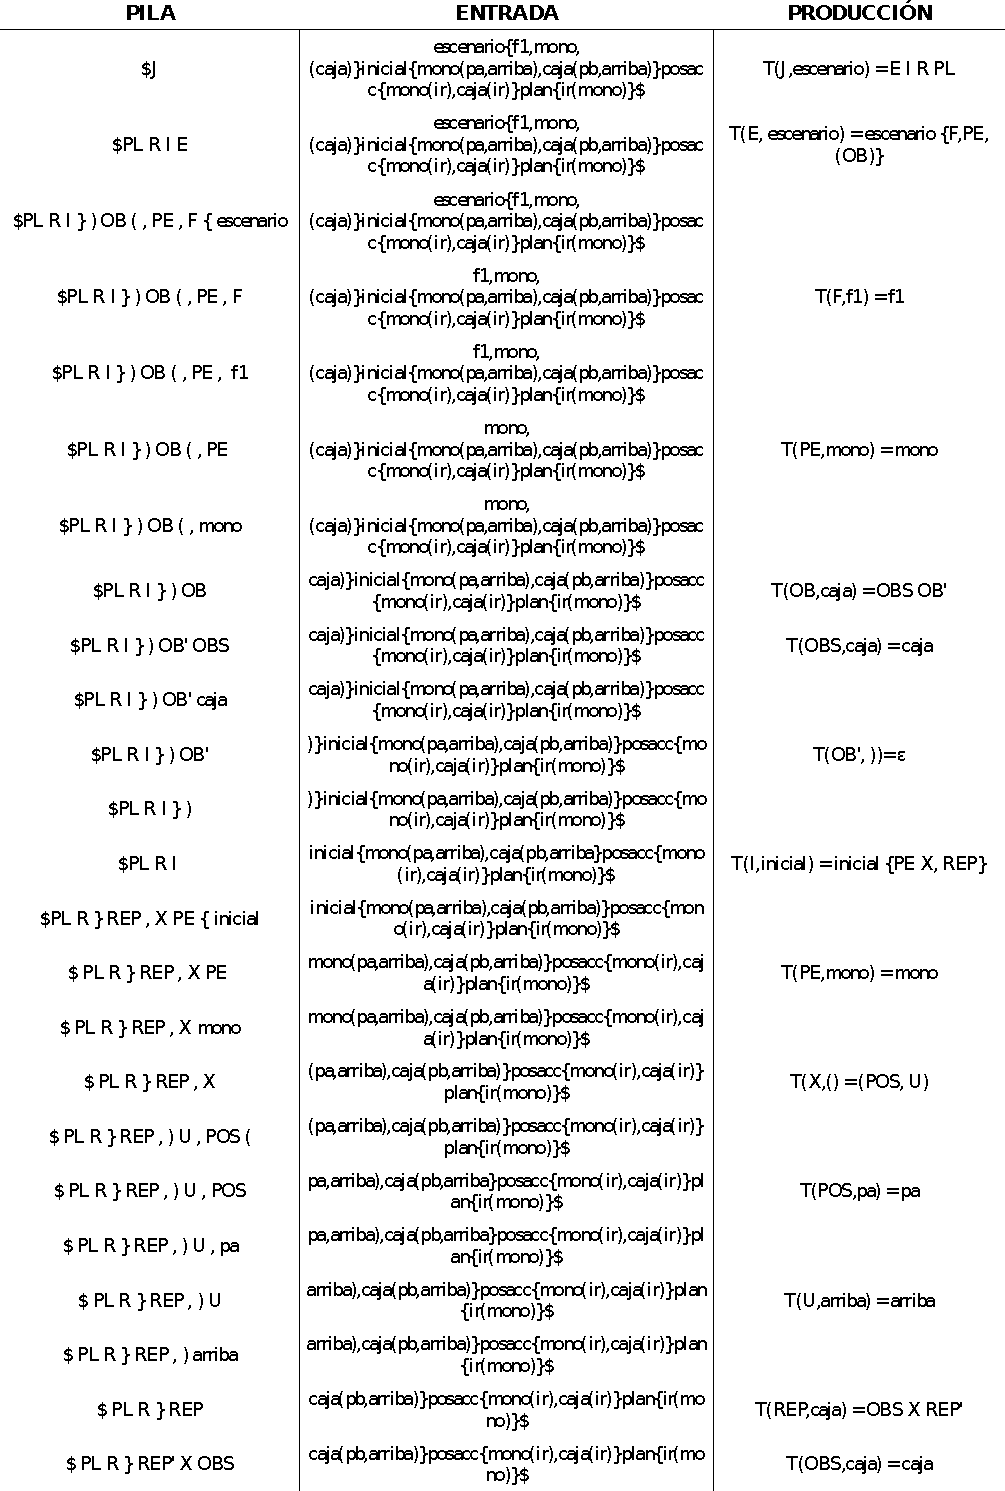
\includegraphics[width=\linewidth]{img/palabra1.pdf}
  \caption{Primera parte de análisis de la cadena.}
  \label{ana1}
\end{figure}

\begin{figure}
  \centering
    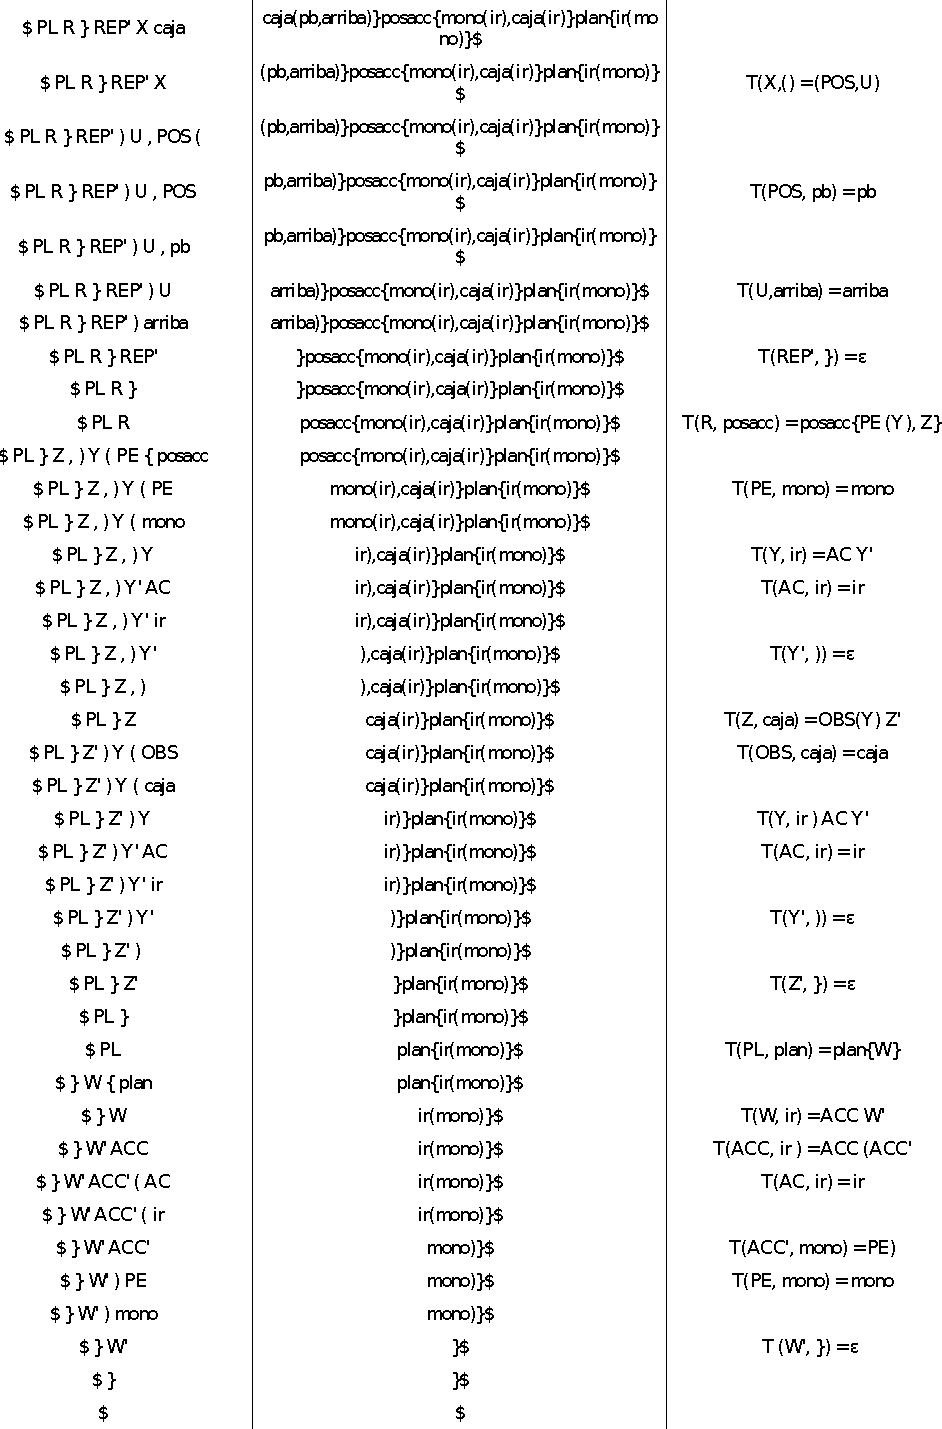
\includegraphics[width=\linewidth]{img/palabra2.pdf}
  \caption{Segunda parte de análisis de la cadena.}
  \label{ana2}
\end{figure}

\end{document}
